\chapter{引言}%
\label{cha:intro}
不断追问组成物质的基本粒子和深入研究粒子之间的相互作用是粒子物理的主旋律。
电子是第一个被发现的亚原子粒子,打破了组成可见物质的基本单元是原子这一传统认识。
发现电子的历史曲折而艰难。
在1858年德国物理学家尤利乌斯·普吕克进行低压气体放电研究的过程中发现
阴极对面的玻璃壁上闪烁着绿色的辉光,看来像是从阴极发出一种看不见的射线,
这被人们称之为``阴极射线``\cite{Segr1981From}。
关于阴极射线的本质,当时在国际上存在两种截然不同的观点。
大多数英国物理学家(如约瑟夫·约翰·汤姆逊)
认为阴极射线是一种带电的粒子流,而赫兹在实验后发现阴极射线未在磁场
中发生偏转,据此认为阴极射线是不带电的。赫兹的实验结果引起了
英国剑桥大学卡文迪许实验室的约瑟夫·约翰·汤姆森的质疑,
在1897,汤姆森重做了赫兹的实验, 这次他使用真空度更高的真空管和更强的电场,
惊奇的是,他观察到阴极射线在磁场中发生了偏转,并计算出阴极射线粒子的质量-电荷比例。
他采用1891年乔治·斯托尼所起的名字——电子来称呼这种粒子。
至此,电子成为了第一个亚被人类发现的亚原子粒子,此时寻找亚原子粒子的序幕被缓缓拉开。

在这个轰轰烈烈的物理学革命中,一个重要的事件是质子的内部结构被发现了,
巧合是这次电子成为了最得力助手。揭示质子内部结构的实验正是
电子-核子深度非弹性散射实验。
\begin{figure}[htpb]
    \centering
    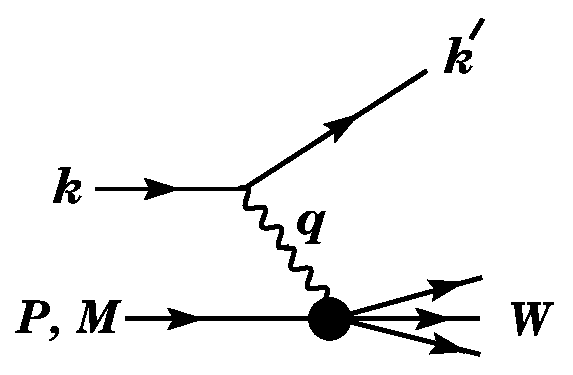
\includegraphics[width=0.8\linewidth]{intr/leptoprod.eps}
    \caption{轻子-核子散射过程示意图。}%
    \label{fig:leptoprod}
\end{figure}
电子-核子的非弹性散射过程$l N \to l X$如图\ref{fig:leptoprod}所示,
$k$和$k'$分别是入射和出射的电子的动量,通过
传播子$\gamma$, $W$或$Z$将动量$q=k-k'$传递给核子,
核子则蜕变为一簇强子。我们将
初态核子的动量记为$P$,末态强子的动量总和记为$W$。
实验上,$x$和$y$是经常被用到的无量纲的物理量,被称为Bjorken变量,
它们的定义为:
\begin{itemize}
    \item $x= \frac{Q^{2} }{2 M \nu}$,式中$Q^2 = - q^2$,
        $\nu$为电子和核子质心系下的能量损失。
        $x$物理意义为被撞的部分子携带的核子动量的比例。
    \item $y = \frac{q.P}{k.P} = \frac{\nu}{E}$,
        物理意义为电子在核子质心系下的能量损失比例。
\end{itemize}
    当$Q^{2} \gg M^{2}$时图示的过程为深度非弹性散射过程,其微分散射截面~\cite{Blumlein:1996vs,Forte:2001ph,Anselmino:1993tc}
的一般形式为
\begin{equation}
\frac{d^2 \sigma^i} {dx dy} 
    = \frac{4 \pi \alpha^2}{xy Q^2} \eta^{i}
    {(1-y - \frac{x^2 y^2 M^2}{Q^2}) F_{2}^{i}
+ y^2 x F_{1}^{i} \mp (y- \frac{y^2}{2}) x F_{3}^{i}
},
\end{equation}
\begin{figure}[htpb]
    \centering
    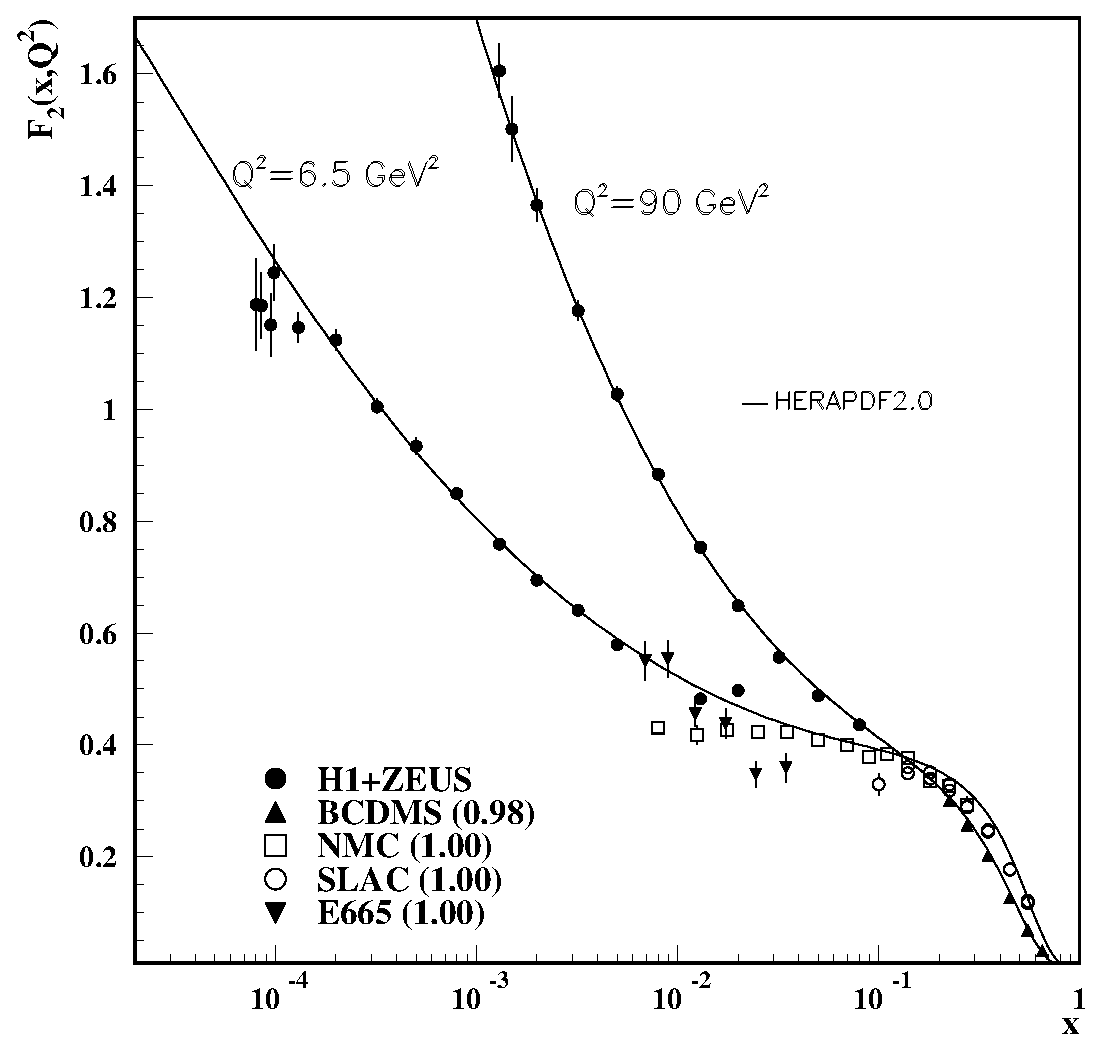
\includegraphics[width=0.8\linewidth]{intr/f2vsx.eps}
    \caption{结构函数的实验测量结果。}%
    \label{fig:f2vsx}
\end{figure}
和核子的内部结构紧密相关,一般的用形状因子$F(x, Q^2)$来描述。
图\ref{fig:f2vsx}展示了$F_{2}$的两组实验测量结果,分别
选取$Q^{2}=6.5,90$ GeV。$F_2$的相关定义见文献\cite{Klein:1983vs}
在$x$极小的区域,即$x<0.1$, $F_{2}$对$Q^2$的依赖较强,然而在$x$较大的区域,
即电子能量损失比较大时,$F_2$几乎不依赖与电子的入射能量,这意味着电子行为在一定程度上与其能量无关,
这就是所谓的标度无关现象。
标度无关的概念最早由James Daniel Bjorken提出\cite{Bjorken:1968dy}.
标度无关现象激起了当时对核子结构的热烈探讨,其中费曼提出的部分子模型(parton
model)是最著名也是最富有成效的,强有力的支持了夸克模型,这个由盖尔曼在1964年提出
的模型,这里的部分子就是盖尔曼模型中的夸克\cite{Greenberg:1981zv}。

图\ref{fig:fix_collider_kineplane}展示了各个实验所长,
\begin{figure}[htpb]
    \centering
    \includegraphics[width=0.8\linewidth]{intr/fix_collider_kineplane.eps}
    \caption{各个实验及能区。}%
    \label{fig:fix_collider_kineplane}
\end{figure}
将图\ref{fig:leptoprod}所示的过程旋转$90^{\circ}$就是另一种研究核子结构的实验手段,
即对撞机实验$e^{+} e^{-} \to N X$,其中最特殊的一种过程是$ e^+ e^- \to B \bar{B}$,
即末态是一对正反重子。
其中的一个打靶实验所不能的优势方面是能够研究超短寿命重子的结构函数,比如超子家族。
$\Lambda$是第一个被实验发现的超子,也是质量最轻的超子,如图所示,它留下的痕迹就是
一个``$\Lambda$``形状。在此之后,
重子八重态家族的其他成员$\Sigma$, $\Xi$, $\Omega$也陆续地被发现。
幸运的是所有的八重态重子都能在正负电子对撞机上成对产生,且产额可观,来源众多。
以BESIII为例,BESIII合作组在2009年和2012年间共取得了13亿的$J/\psi$
样本,主要的正反重子对的产额列举在表\ref{tab:bbar_production}中
 \begin{table}[htpb]
     \caption{BESIII上的正反重子对产额。只考虑$J/\psi$样本}%
     \label{tab:bbar_production}
     \centering
     \begin{tabular}{p{0.4\linewidth}
         p{0.25\linewidth}<{\centering}c
         p{0.25\linewidth}<{\centering}c }
         \toprule[0.2em]
         Decay mode & $\mathcal{B}(\times 10^{-3})$ & $N_{B} (\times
         10^{6})$ \\
         \midrule
         $J/\psi \to \Lambda \bar{\Lambda}$ & $1.61 \pm 0.15$ &
         $1.61 \pm 1.5$ \\
         $J/\psi \to \Sigma^{0} \bar{\Sigma}^{0}$ & $1.29 \pm 0.09$ &
         $12.9 \pm 0.9$ \\

         $J/\psi \to \Sigma^{+} \bar{\Sigma}^{-}$ & $1.50 \pm 0.24$ &
         $15.0 \pm 2.4$ \\

         $J/\psi \to \Xi^{-} \bar{\Xi}^{+}$ & $0.86 \pm 0.11$ &
         $8.6 \pm 1.0$ \\

         $J/\psi \to \Xi^{0} \bar{\Xi}^{0}$ & $1.20 \pm 0.24$ &
         $12.0 \pm 2.4$ \\
         $\psi(2S) \to \Omega \bar{\Omega} $ & $0.05 \pm 0.01$ &
         $0.15 \pm 0.03$ \\
         \bottomrule
     \end{tabular}
\end{table}
此时一个引人入胜的问题除了$c\bar{c}$共振态,正反重子对的产生是否还有其他来源?
一个备选的选项是奇异粲介子,
本文选定了标准模型允许的衰变过程$D_{s}^{+} \to p \bar{p} e^{+} \nu_{e}$
来寻找这种来源,相关的研究在后续的章节中有详细的描述。
另一个独特优势是借助于末态重子的极化信息能够获得更多的结构函数细节。
在$3.0~{\rm GeV}$能区,电子和超子的电磁相互作用起主导,
我们常用电磁形状因子$G_{E}(G_{M})$来称呼光子做传播子时的结构函数,此时的
散射类型为非弹性散射。一般的,散射振幅的形式为
\begin{equation}
    \begin{split}
        \frac{d\sigma}{d \cos\theta}  \sim & 1+ \alpha _{\psi } \cos^2\theta
        + \sin ^2\theta \hat{s}_{1}^x \hat{s}_{2}^x
        + \alpha_{\psi} \sin^2\theta \hat{s}_{1}^y \hat{s}_{2}^y 
        - \left( \alpha_{\psi} +\cos^2 \theta  \right)\hat{s}_{1}^z
        \hat{s}_{2}^z \\
        &+ \sqrt{1-\alpha_{\psi}^2} \cos\Phi  \sin\theta 
          \cos\theta
        \left( \hat{s}_{1}^x \hat{s}_{2}^z  - \hat{s}_{1}^z \hat{s}_{2}^x\right)
        +\sqrt{1-\alpha _{\psi}^2}
        \sin\Phi  \sin\theta \cos\theta  (\hat{s}_{1}^y - \hat{s}_{2}^y),
    \end{split}
    \label{eq:BBbar_amplitude}
\end{equation}
式中
\begin{equation}
    \alpha_{\psi} \equiv \frac{s |G_{M}|^{2} -4 m^{2} |G_{E}|^{2} }
    {s|G_{M}|^{2} + 4 m^{2}|G_{E}|^{2}},
\end{equation}
需要特别指出,只有当电磁形状因子$G_{E}$与$G_{M}$之间存在相位差时才能独立测量两个超子的衰变常数。
而末态超子的极化强度与相位差的正弦成正比,极化为
\begin{equation}
    P^{y}_{B} = \frac{\sqrt{1 - \alpha_{\psi}^{2}} \sin \Phi
    \sin \theta \cos \theta}
    {1+ \alpha_{\psi} \cos^{2} \theta}
\end{equation}
在 2018 年 BESIII 合作组\cite{Ablikim:2018zay}对 $J/\psi \to \Lambda \bar{\Lambda}$的事例进行拟合,
发现 $\Lambda$ 是部分极化的,观测到的极化强度随极角的分布为
\begin{figure}[htpb]
    \centering
    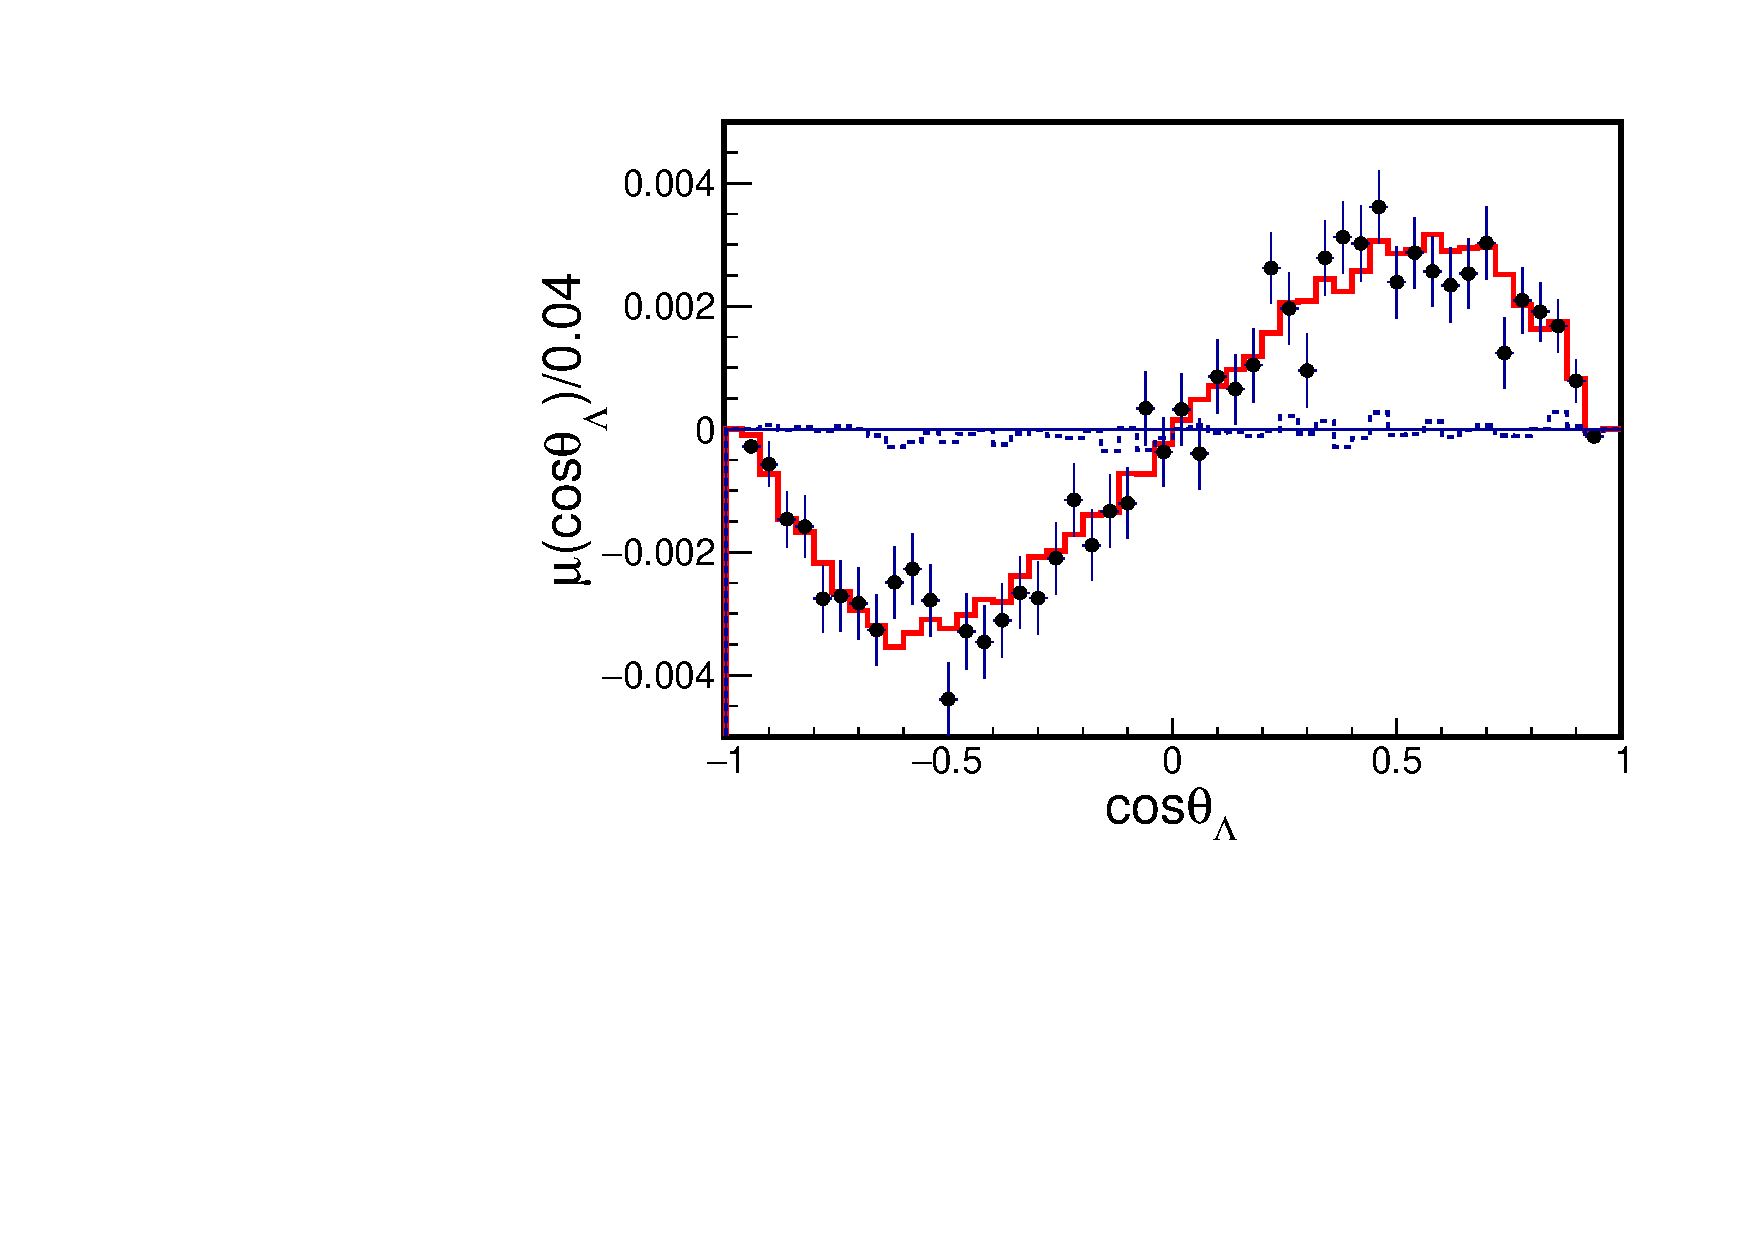
\includegraphics[width=0.9\linewidth]{intr/figPNa.pdf}
    \caption{末态$\Lambda$的极化强度随极角的变化而变化。}%
    \label{fig:figPNa}
\end{figure}
对八重态的成员进行一系列的研究迫切而重要,这也是本文选题动机的原因之一。
将图\ref{fig:leptoprod}中的入射轻子旋转$180$°则又一种研究结构函数的方式,即通过超子的衰变过程
$B' \to B l^{+} l^{-}$,这相应于$Q^{2}$极小的情形,即结构函数在零点时的行为。
一个理想的过程是$\Sigma^{0} \to \Lambda e^{+} e^{-}$,在几个超子的达利兹衰变中,
这个分支比最大,理论预期为$0.5\%$,这两项研究结合在以前将充分利用的对撞机产生的
$\Sigma^{0} \bar{\Sigma}^{0}$样本,这是本文选题的另一个重要原因。 
在接下来的章节里,将首先研究重子对的产生过程,包括粲介子中正反质子对的产生(第章),
$c\bar{c}$共振态$J/\psi$和$\psi(2S)$中$\Sigma^{0}\bar{\Sigma}^{0}$的产生,并详细的
测量了实验的衰变参数,包括$\alpha_{\psi}$,$\Delta \phi$, $\alpha_{\Lambda}$, $\alpha_{\bar{\Lambda}}$,
和$\alpha_{\gamma}$,并在此基础了谈论了在$\Sigma$衰变过程中的P、C和P宇称守恒
接着文章讨论了
磁场对实验测量的潜在影响并做了数值估计,最后本文研究了$\Sigma^{0}$的达利兹衰变过程
$\Sigma^{0} \to \Lambda e^{+} e^{-}$。


